\documentclass{../khlslides}


\title[Algo1]{Introductie}
\author{Fr\'ed\'eric Vogels}

\newcommand{\jscodeblock}[3][]{\begin{block}{#3}\lstinputlisting[language=javascript,#1]{#2}\end{block}}
\newcommand{\X}[2]{\tikz[baseline,remember picture]{\node[anchor=base,inner sep=0mm] (#2) {{#1}};}}


% Segmented pie chart
% \pgfkeys{/mylib/segpie/.cd,
%          fill/.store in=\fill,
%          inner radius/.store in=\innerradius,
%          outer radius/.store in=\outerradius}

\pgfkeys{/mylib/segpie/.cd,
         fill/.initial=white,
         inner radius/.initial=0,
         outer radius/.initial=1
       }

\newcommand{\segpie}[4][]{
  {
    \newcommand{\segment}[3][]{
      {
        \pgfkeys{/mylib/segpie/inner radius/.get=\innerradius}
        \pgfkeys{/mylib/segpie/outer radius/.get=\outerradius}
        \pgfkeys{/mylib/segpie/fill/.get=\fill}
        \pgfmathparse{##2/##3*360}\let\fromangle\pgfmathresult
        \pgfmathparse{(##2+1)/##3*360}\let\toangle\pgfmathresult
        \draw[thin,fill=\fill] (\fromangle:\innerradius) --
                               (\fromangle:\outerradius) --
                               (\toangle:\outerradius) --
                               (\toangle:\innerradius) --
                               cycle;
      }
    }
    \pgfkeys{/mylib/segpie/.cd,#1}
    \foreach \idx in {#2,...,#3} {\segment{\idx}{#4}};
  }
}



\begin{document}

\maketitle

\section{Introductie}

\frame{ \tableofcontents[currentsection] }

\begin{frame}
  \frametitle{Studiebelasting}
  \begin{columns}
    \column{.5\textwidth}
    \begin{center}
      \begin{tikzpicture}
        \pgfkeys{/mylib/segpie/.cd, inner radius=1.5, outer radius=2.5}
        \only<1>{
          \segpie[fill=white]{0}{74}{74}
        }
        \only<2>{
          \segpie[fill=red]{0}{11}{74}
          \segpie[fill=white]{12}{74}{74}
        }
        \only<3>{
          \segpie[fill=red]{0}{11}{74}
          \segpie[fill=blue]{12}{29}{74}
          \segpie[fill=white]{30}{74}{74}
        }
        \only<4>{
          \segpie[fill=red]{0}{11}{74}
          \segpie[fill=blue]{12}{29}{74}
          \segpie[fill=green]{30}{74}{74}          
        }
      \end{tikzpicture}
    \end{center}
    \column{.5\textwidth}
      \begin{itemize}
        \item<1-> 3 studiepunten
        \item<1-> 25 uur per studiepunt
        \item<1-> 12 weken
        \item<1-> $\Rightarrow$ 75 uren in totaal
        \item<2-> {\color{red} 1 uur/week theorie}
        \item<3-> {\color{blue} 1.5 uur/week oefeningen}
        \item<4-> {\color{green} 45 uur zelfstudie}
      \end{itemize}
  \end{columns}
\end{frame}

% \begin{frame}
%   \frametitle{Puntenverdeling}
%   \begin{columns}
%     \column{.5\textwidth}
%     \begin{itemize}
%       \item {\color{red} 40\%: opdrachten}
%              \begin{itemize}
%                \item {\color{red} Toetsen}
%              \end{itemize}
%              \vskip4mm
%       \item {\color{blue} 60\%: examen}
%              \begin{itemize}
%                \item {\color{blue} 10\% mondeling contactexamen}
%                \item {\color{blue} 50\% schriftelijk contactexamen}
%              \end{itemize}
%     \end{itemize}
%     \column{.5\textwidth}
%     \begin{center}
%       \begin{tikzpicture}
%         \pgfkeys{/mylib/segpie/.cd, inner radius=1.5, outer radius=2.5}
%         \segpie[fill=red]{0}{3}{10}
%         \segpie[fill=blue]{4}{9}{10}
%       \end{tikzpicture}
%     \end{center}
%   \end{columns}
%   \vskip5mm
%   {\tiny (Offici\"ele informatie te vinden op studiewijzer)}
% \end{frame}

\begin{frame}
  \frametitle{Plaatsing}
  \begin{center}
    \begin{tikzpicture}[vak/.style={rectangle,draw=black,fill=blue!25,thin,minimum size=12mm},
                        arr/.style={->,thick},
                        sem/.style={left color=blue!75, right color=blue!25,drop shadow},
                        semc/.style={rotate=90,fill=blue!75,rectangle,drop shadow},
                        lang/.style={circle,fill=red!50,circular drop shadow},
                        langarr/.style={ultra thick,->,red!50}]
      \path[use as bounding box] (-3,0) rectangle (3,5);
      \node[semc] at (-2.25,3.75) {S1};
      \node[semc] at (-2.25,1.75) {S2};
      \node[semc] at (-2.25,-0.25) {S3};
      \shade[sem] (-2,4.75) rectangle (2, 3.25);
      \shade[sem] (-2,2.75) rectangle (2, 1.25);
      \shade[sem] (-2,0.75) rectangle (2, -0.75);
      \node[vak] (bop)    at (-1,4)   {BOP};
      \node[vak] (algo1)  at (1,4)    {Algo1};
      \node[vak] (oop)    at (-1,2)   {OOP};
      \node[vak] (algo2)  at (1,2)    {Algo2};
      \node[vak] (ooo)    at (-1,0)   {OOO};
      \draw[arr] (algo1) -- (bop);
      \draw[arr] (bop) -- (oop);
      \draw[arr] (oop) -- (ooo);
      \draw[arr] (algo1) -- (algo2);
      \draw[arr] (bop) -- (algo2);

      \only<2>{
        \node[lang] (java) at (-4,2.5) {Java};
        \node[lang] (javascript) at (3.75,4) {JavaScript};
        \draw[langarr] (java) to [bend left=45] (bop);
        \draw[langarr] (java) to [bend left=45] (algo2);
        \draw[langarr] (java) to [bend left=45] (oop);
        \draw[langarr] (java) to [bend left=45] (ooo);
        \draw[langarr] (javascript) to [bend right=45] (algo1);
      }
    \end{tikzpicture}
  \end{center}
\end{frame}

%%% Local Variables: 
%%% mode: latex
%%% TeX-master: "intro"
%%% End: 

\section{Algoritmes}

\frame{ \tableofcontents[currentsection] }

\begin{frame}
  \frametitle{Vierkantswortel}
  \structure{Definitie}
  \[
    y = \sqrt{x} \quad\iff\quad y^2 = x
  \]
  \vskip5mm
  \structure{Voorbeelden}
  \[
    \begin{array}{rcl}
      \sqrt1 & = & 1 \\
      \sqrt4 & = & 2 \\
      \sqrt9 & = & 3 \\
             & \vdots & \\
      \sqrt{100} & = & 10 \\
      & \visible<2>{\vdots} \\
      \visible<2>{\sqrt{1000}} & \visible<2>{=} & \visible<2>{?}
    \end{array}
  \]
\end{frame}


\begin{frame}
  \frametitle{Vierkantswortel}
  \code[font size=\small,width=.95\linewidth]{sqrt.js}
\end{frame}

\begin{frame}
  \frametitle{Algorithms: They're Everywhere}
  \begin{center}
    \begin{tikzpicture}[box/.style={fill=red,opacity=.25,ultra thick},
                        msg/.style={rectangle,fill=red,opacity=.25,text opacity=1}]
      \path[use as bounding box] (-5,-1) rectangle (5,5);
      \node[anchor=south] (pic) at (0,0) { \pgfimage[width=10cm,interpolate=true]{borderlands.jpg} };
      \only<2>{
        \draw[box] (1, 4.5) circle (1);
        \node[msg,anchor=north] at (0, 0) { \parbox{10cm}{ \centering
            Hidden surface removal \\ {\tiny (Z-buffering, Painter's Algorithm, BSP trees, \dots)}
        }};
      }
      \only<3>{
        \draw[box] (-3, 3) circle (1);
        \draw[box] (1.5, 3) circle (.5);
        \node[msg,anchor=north] at (0, 0) { \parbox{10cm}{ \centering
            Hit detection
        }};
      }
      \only<4>{
        \draw[box] (1.85, 2.3) circle (.75);
        \node[msg,anchor=north] at (0, 0) { \parbox{10cm}{ \centering
            Particle system (fire simulation)
        }};
      }
      \only<5>{
        \draw[box] (0, 2) circle (.9);
        \draw[box] (3.5, 1.2) circle (.9);
        \node[msg,anchor=north] at (0, 0) { \parbox{10cm}{ \centering
            Shadow casting (static vs dynamic)
        }};
      }
      \only<6>{
        \draw[box] (0.3, 2.7) circle (.5);
        \node[msg,anchor=north] at (0, 0) { \parbox{10cm}{ \centering
            Artificial Intelligence \\
            {\tiny (Path Finding: A-star, Game Trees: Minimax, Artifical Neural Networks, \dots)}
        }};
      }
    \end{tikzpicture}
  \end{center}
\end{frame}

\begin{frame}
  \frametitle{Algoritmes}
  \begin{itemize}
    \item Stap-voor-stap beschrijving van oplossingsmethode
          \vskip5mm
    \item Drie ``kwaliteitsmetrieken''
          \begin{itemize}
            \item Algoritme moet ooit eindigen
            \item Algoritme moet correct resultaat opleveren
            \item Algoritme moet zo effici\"ent mogelijk werken
          \end{itemize}
          \vskip5mm
    \item Knelpunten
          \begin{itemize}
            \item Enige creativiteit vereist
            \item Randgevallen
            \item Begrijpen van de details
          \end{itemize}
  \end{itemize}
\end{frame}

\begin{frame}
  \frametitle{Puzzel}
  \begin{center}
    \begin{tikzpicture}
      \node { \pgfimage[width=5cm,interpolate=true]{scale.png} };
    \end{tikzpicture}
  \end{center}  
  \begin{overprint}
    \onslide<1>
    \structure{Probleemstelling}
    \begin{itemize}
      \item Gegeven 9 identiek uitziende goudmunten
      \item E\'en ervan is vals, deze is wat lichter
      \item Vind de valse munt met zo weinig mogelijk wegingen
    \end{itemize}

    \onslide<2>
    \structure{Na\"ieve oplossing}
    \begin{itemize}
      \item Telkens twee munten met elkaar vergelijken
      \item Een lichtere gevonden $\rightarrow$ valse munt gevonden
      \item Kan tot 7 wegingen leiden
    \end{itemize}

    \onslide<3>
    \structure{Effici\"entste oplossing}
    \begin{itemize}
      \item Drie munten met drie andere vergelijken
      \item Indien gelijk: valse zit in laatste drie
      \item Anders: kies de lichtste drie
      \item Slechts 2 wegingen nodig
    \end{itemize}

  \end{overprint}
\end{frame}

\begin{frame}
  \frametitle{Overzicht Cursus}
  \begin{enumerate}
    \item Variabelen
    \item Conditionele Logica
    \item Lussen
    \item Functies
    \item Recursie
    \item Rijen
    \item Sorteeralgoritmen
    \item Complexiteit
  \end{enumerate}
\end{frame}


%%% Local Variables: 
%%% mode: latex
%%% TeX-master: "intro"
%%% End: 

\section{HTML \& JavaScript}

\frame{ \tableofcontents[currentsection] }


\begin{frame}
  \frametitle{HTML}
  \begin{center}
    \begin{tikzpicture}[remember picture]
      \path[use as bounding box] (-2.5,-4) rectangle (8,3);

      \node[draw,rectangle split,rectangle split parts=2,inner sep=1mm,anchor=north] (html) at (3,3) {
        {\sc example.html}
        \nodepart{second}
        \inlinecode[language=HTML,font size=\tiny,width=.75\linewidth,frame=none]{example.html}
      };
      \node[draw,anchor=south west,inner sep=1mm,fill=white,rectangle split,rectangle split parts=2] at (-2.5,-4) {
        {\sc resultaat}
        \nodepart{second}
        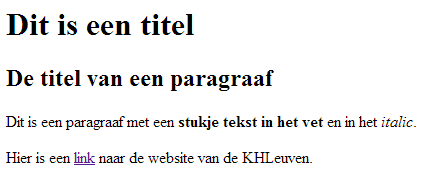
\includegraphics[width=4.5cm]{raw-html.png}
      };
    \end{tikzpicture}
  \end{center}
\end{frame}

\begin{frame}
  \frametitle{HTML+CSS}
  \begin{center}
    \begin{tikzpicture}[remember picture]
      \path[use as bounding box] (-2.5,-4) rectangle (8,3);

      \node[draw,rectangle split,rectangle split parts=2,inner sep=1mm,anchor=north] (html) at (3,3) {
        {\sc example.html}
        \nodepart{second}
        \inlinecode[language=HTML,font size=\tiny,width=.75\linewidth,frame=none]{example2-tex.html}
      };
      \node[draw,fill=white,rectangle split,rectangle split parts=2,anchor=north west,inner sep=1mm] (css) at ($ (html.north west) + (4,-2) $) {
        {\sc example.css}
        \nodepart{second}
        \inlinecode[language=CSS,font size=\tiny,width=.4\linewidth,frame=none]{example.css}
      };
      \draw[->,thick] (csslink.east) to[bend left=30] (css.north);
      \node[draw,anchor=south west,inner sep=1mm,fill=white,rectangle split,rectangle split parts=2] at (-2.5,-4) {
        {\sc resultaat}
        \nodepart{second}
        
\includegraphics[width=4.5cm]{html-css.png}
      };
    \end{tikzpicture}
  \end{center}
\end{frame}

\begin{frame}
  \frametitle{HTML+CSS+JavaScript}
  \begin{center}
    \begin{tikzpicture}[remember picture]
      \path[use as bounding box] (-2.5,-4) rectangle (8,3);

      \node[draw,rectangle split,rectangle split parts=2,inner sep=1mm,anchor=north] (html) at (3,3) {
        {\sc example.html}
        \nodepart{second}
        \inlinecode[language=HTML,font size=\tiny,width=.75\linewidth,frame=none]{example3-tex.html}
      };

      \node[draw,fill=white,rectangle split,rectangle split parts=2,anchor=north west,inner sep=1mm] (css) at ($ (html.north west) + (4,-2) $) {
        {\sc example.css}
        \nodepart{second}
        \inlinecode[language=CSS,font size=\tiny,width=.4\linewidth,frame=none]{example.css}
      };
      \draw[->,thick] (csslink.east) to[bend left=30] (css.north);

      \node[draw,fill=white,rectangle split,rectangle split parts=2,anchor=north west,inner sep=1mm] (js) at ($ (css.north west) + (1,-2) $) {
        {\sc example.js}
        \nodepart{second}
        \inlinecode[language=javascript,font size=\tiny,width=.4\linewidth,frame=none]{example.js}
      };
      \draw[->,thick] (jslink.south) to[bend right=30] (js.west);

      \node[draw,anchor=south west,inner sep=1mm,fill=white,rectangle split,rectangle split parts=2] at (-2.5,-4) {
        {\sc resultaat}
        \nodepart{second}
        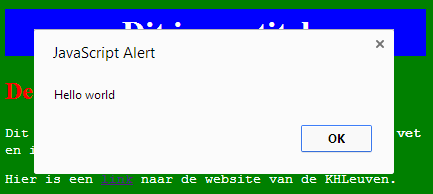
\includegraphics[width=4.5cm]{html-css-js.png}
      };
    \end{tikzpicture}
  \end{center}
\end{frame}

\begin{frame}
  \frametitle{Sjabloon}
  \begin{center}
    \begin{tikzpicture}
      \node[draw,rectangle split,rectangle split parts=2,inner sep=1mm,anchor=north] (html) {
        {\sc html}
        \nodepart{second}
        \inlinecode[language=HTML,font size=\tiny,width=.75\linewidth,frame=none]{template.html}
      };

      \node[draw,rectangle split,rectangle split parts=2,inner sep=1mm,anchor=north] (javascript) at ($ (html.south) + (0,-.5) $)  {
        {\sc code.js}
        \nodepart{second}
        \inlinecode[language=HTML,font size=\tiny,width=.75\linewidth,frame=none]{template.js}
      };
    \end{tikzpicture}
  \end{center}
\end{frame}

\begin{frame}
  \frametitle{Voorbeeld}
  \begin{center}
    \begin{tikzpicture}
      \node[draw,rectangle split,rectangle split parts=2,inner sep=1mm,anchor=north] (html) {
        {\sc html}
        \nodepart{second}
        \inlinecode[language=HTML,font size=\tiny,width=.75\linewidth,frame=none]{template.html}
      };

      \node[draw,rectangle split,rectangle split parts=2,inner sep=1mm,anchor=north] (javascript) at ($ (html.south) + (0,-.5) $)  {
        {\sc code.js}
        \nodepart{second}
        \inlinecode[language=javascript,font size=\tiny,width=.75\linewidth,frame=none]{code.js}
      };

      \node[anchor=north east,inner sep=1mm,fill=white] at (-.5,-5) {
        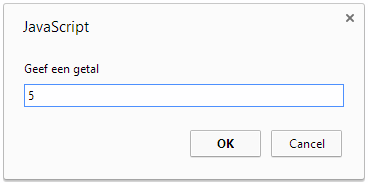
\includegraphics[width=4cm]{input.png}
      };
      \node[anchor=north west,inner sep=1mm,fill=white] at (.5,-5) {
        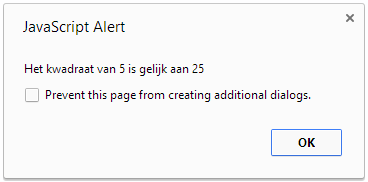
\includegraphics[width=4cm]{output.png}
      };
    \end{tikzpicture}
  \end{center}
\end{frame}


%%% Local Variables: 
%%% mode: latex
%%% TeX-master: "intro"
%%% End: 



\end{document}



%%% Local Variables: 
%%% mode: latex
%%% TeX-master: t
%%% End: 
